\newpage

\section{Hauptteil} \label{hauptteil}
Einleitende Worte zum Hauptteil.
\subsection{Architektur} \label{architektur}
Server
Frontend API Backend
Shopify

\begin{figure}[H]
    \centering
    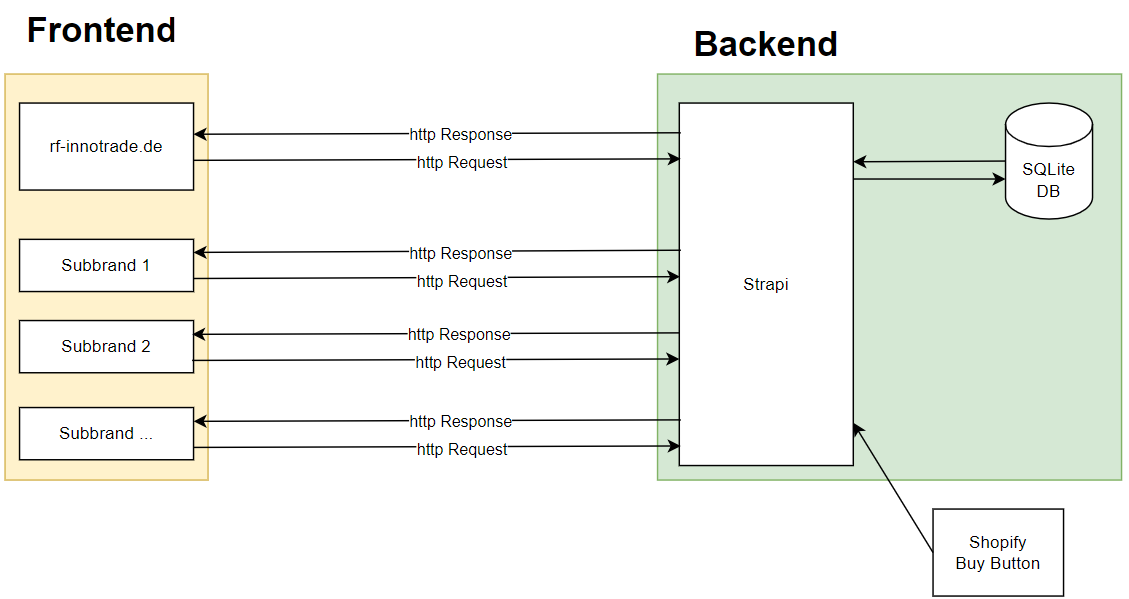
\includegraphics[width=1\textwidth]{figures/architektur.png}
    \caption{Architektur Schaubild, Quelle: Eigene Darstellung}
	\label{fig:architekturSchaubild}
\end{figure}

\subsection{Strapi als Backend} \label{strapiMain}
Strapi bietet von Haus aus eine gute Grundstruktur. Alle notwendigen Dateien werden von Strapi grundlegend mitgeliefert und müssen im Anschluss nur noch an die individuellen Anforderungen angepasst werden. In diesem Kapitel werden wir auf die von uns veränderten und auf unsere Bedürfnisse zugeschnittenen Dateien eingehen und deren Funktionalitäten erläutern.
\subsubsection{Vite.config.js} \label{viteconfigjs}
Diese Datei ist abgelegt unter: „rfinnotrade/strapi/src/admin/vite.config.js“.
Um zu erläutern, was in dieser Datei passiert, muss das grundlegende Prinzip von Cross-Origin Ressource Sharing (CORS) verstanden werden. CORS ist ein Sicherheitsmechanismus, welcher in Webbrowsern verwendet werden kann, um Zugriff auf Ressourcen von einer anderen Domain kontrolliert zulassen zu können. Daher auch der Begriff „Cross-Origin“. Es handelt sich hierbei um eine Erweiterung der standardmäßig verwendeten Same-Origin-Policy (SOP), welche Zugriffe nur von der selben Domain zulässt (Vgl. Cross-Origin Resource Sharing – Wikipedia, o. J.). In unserem Fall erlaubt diese Struktur also den Fremdzugriff auf Ressourcen innerhalb von Strapi.
Diese Datei wird ebenfalls grundsätzlich von Strapi mitgeliefert und wurde von uns leicht angepasst.

\begin{lstlisting}[language=JavaScript, caption={Vite.config.js}, label={lst:viteconfigjs}]
const { mergeConfig } = require('vite');

module.exports = (config) => {
  // Important: always return the modified config
  return mergeConfig(config, {
    resolve: {
      alias: {
        '@': '/src',
      },
    },
    server: {
      cors: {
        origin: true,
        credentials: true,
      },
    },
  });
};
\end{lstlisting}

In Zeile 13 und 14 erlauben wir den Zugriff auf Strapi und legen zudem fest, dass credentials weitergeleitet werden sollen. Hier könnte man auch weitere Restriktionen vornehmen, was von uns allerdings in der Datei „Middleware.js“ vorgenommen wurde.
\subsubsection{Middlewares.js} \label{middlewares}
Diese Datei liegt unter „rfinnotrade/strapi/config/middleware.js“.
Der Begriff Middleware in unserem Webprojekt ist als eine Softwareschicht zwischen unserer Webanwendung und dem Server zu verstehen. Die Middleware verarbeitet dabei eingehende Anfragen und ausgehende Antworten, um zum Beispiel Login- und Authentifizierungsfunktionen zu ermöglichen.
HIER CODE EINFÜGEN
Die hier gezeigte Middleware.js, arbeitet die aufgeführten Middleware-Funktionen nacheinander und in genau dieser Reihenfolge ab. Somit wird sichergestellt, dass aufeinander aufbauende Funktionen auch in der richtigen Reihenfolge ausgeführt werden. Es ist außerdem noch wichtig zu erwähnen, dass dies Strapi Middleware-Funktionen sind, da wir uns nach wie vor innerhalb unserer Strapi Konfiguration befinden.
Neben der Anmeldung unter unserer rf-innotrade.de Admin Seite oder für andere API-Calls, welche nur von einem angemeldeten Admin durchgeführt werden dürfen, ist diese Datei für die im vorherigen Kapitel erwähnte CORS-Konfiguration zuständig.
HIER CODE EINFÜGEN, ZEILE 6-16
Diese Konfiguration sorgt dafür, dass Authentifizierungsanfragen immer nur über die in Zeile 9 genannten Domains erlaubt sind und die Anfrage nur dann weiterverarbeitet werden darf.

\subsubsection{Token.js} \label{token}
Die nächste Datei ist unter dem Pfad „rfinnotrade/strapi/src/middlewares/Token.js“ abgelegt.
Diese Datei ist ebenfalls sehr wichtig, da Strapi von Haus aus keine Cookies verarbeiten kann. Die Verarbeitung von Cookies ist in unserem Fall notwendig, damit Informationen wie der aktuelle Login-Status oder welcher User, mit welchen Berechtigungen, startet gerade eine Anfrage an Strapi, abgefragt werden können.
HIER CODE EINFÜGEN
Realisiert wird diese Funktion im ersten Schritt durch das Auslesen des Cookies aus dem mitgelieferten Gesamtkontext der Webseite in Zeile 2 und 3. Im nächsten Schritt wird in den Zeilen 6 bis 8 der JSON Web Token (JWT) extrahiert. Sollte die Abfrage für ein JWT erfolgreich sein, wird in Zeile 9 und 10 das Token um „Bearer“ erweitert und dem „Authorization-Header“ des Webseitenkontextes wieder hinzugefügt.
Durch diese Middleware Funktion versteht Strapi, ob ein User berechtigter Weise eingeloggt ist oder Serveranfragen durchführen darf.
\subsubsection{Custom.js} \label{custom}
Die nachfolgende Datei liegt unter „rfinnotrade/strapi/src/api/custom/controllers/custom.js“ und beinhaltet verschiedene Funktionen. Im Folgenden werde ich auf die Funktionen „login“, „logout“ und „checkAuthStatus“ eingehen, da diese im Kontext von Strapi und den bisher genannten Funktionen am relevantesten sind.

Als erstes gehen wir auf die Login-Funktion ein. Diese Funktion erledigt die Aufgabe, den eigentlichen Login bei einer Login-Anfrage von der Admin Seite zu verifizieren, Daten aus Strapi abzufragen und darüber hinaus alle notwendigen Daten in den Cookies zu setzen.

\begin{lstlisting}[language=JavaScript, caption={Login-Funktion}, label={lst:customjsLogin}]
async login(ctx) {
    const { body } = ctx.request;
    const hostname = "localhost";
    const absoluteURL = `http://${hostname}:${strapi.config.server.port}`;
    const sanitizeOutput = (user) => {
      const {
        password,
        resetPasswordToken,
        confirmationToken,
        ...sanitizedUser
      } = user; // be careful, you need to omit other private attributes yourself
      return sanitizedUser;
    };
    try {
      console.log("Tryin to login");
      // Now submit the credentials to Strapi's default login endpoint
      let { data } = await axios.post(`${absoluteURL}/api/auth/local`, body);
      const populatedUser = await strapi.entityService.findOne(
        "plugin::users-permissions.user",
        data.user.id,
        {
          populate: {
            role: {
              fields: ["type"],
            },
          },
        }
      );
      data.user = sanitizeOutput(populatedUser);
      // Set the secure cookie
      if (data && data.jwt) {
        ctx.cookies.set("jwt", data.jwt, {
          httpOnly: true,
          secure: false,
          SameSite: "None",
          maxAge: 1000 * 60 * 60 * 24 * 7, // 7 Day Age
        });
      }
      // Respond with the jwt + user data, but now this response also sets the JWT as a secure cookie
      return ctx.send(data);
    } catch (error) {
      console.log("An error occurred:", error.response);
      return ctx.badRequest(null, error);
    }
  },
\end{lstlisting}

Um diesen Vorgang zu realisieren, wird erneut der gesamte Webseitenkontext in Zeile 1 übergeben und daraus alle „request“-Daten in Zeile 2 geladen. Hier sind unter anderem die Eingaben des Benutzers gespeichert.
Von Zeile 5 bis Zeile 13, wird die Funktion „sanitizeOutput“ deklariert, welche erst später angewendet wird.
Ab Zeile 14 wird versucht mithilfe der übergebenen Login-Daten, eine Anfrage an Strapis eigentliche Login API durchzuführen. Ist diese Anfrage erfolgreich, werden die entsprechenden Benutzerdaten aus der Strapi Datenbank geladen, unter anderem die Benutzerrollen abgefragt.
Ist alles erledigt, wird eine Cookie mit allen notwendigen Informationen zurückgegeben und in den Webseitenkontext geladen.
Somit wurde die Login Abfrage erfolgreich über eine API durchgeführt und alle notwendigen Login Informationen anschließend in den Cookies der Webseite für weiter Abfragen gespeichert. Eine automatische Logout Funktion wurde in Zeile 68 ebenfalls großzügig implementiert. Diese würde spätestens nach 7 Tagen greifen, das Cookie auslaufen und der Logout somit automatisch erfolgen.

Der ebenfalls implementierten Logout-Funktion wird zu Beginn erneut der Webseitenkontext übergeben.

\begin{lstlisting}[language=JavaScript, caption={Logout-Funktion}, label={lst:customjsLogout}]
async logout(ctx) {
    try {
      // Clear the JWT cookie
      ctx.cookies.set('jwt', null, {
        httpOnly: true,
        secure: false,
        maxAge: 0,
      });
      
      return ctx.send({
        message: 'Successfully logged out',
      });
    } catch (error) {
      return ctx.badRequest(null, error);
    }
  },
\end{lstlisting}

In Zeile 4 wird dann zunächst das Cookie aus dem Kontext ausgelesen und und das JWT auf „NULL“ gesetzt, wodurch der Logout theoretisch bereits erfolgt ist. Zusätzlich wird der automatische Logout, welcher in der Login Funktion auf 7 Tage gesetzt wird, auf den Wert 0 gesetzt.
Dadurch löst sich das Cookie selber auf und der Logout würde ebenfalls erfolgen. Das Cookie wird am Ende wieder an den Webseitenkontext zurückgegeben.

Die Funktion checkAuthStauts hat die Aufgabe, den aktuellen Login Status bei Aufruf dieser Funktion abzufragen. Diese Funktion ergänzt die Login- und Logout-Funktion also um eine weiter wichtige Funktionalität.
Die Funktion ist ähnlich aufgebaut wie Login und Logout.

\begin{lstlisting}[language=JavaScript, caption={checkAuthStatus-Funktion}, label={lst:customjsCheckAuthStatus}]
async checkAuthStatus(ctx) {
    // Check for JWT in cookies first
    const jwtCookie = ctx.cookies.get('jwt');
    
    if (!jwtCookie) {
      return ctx.unauthorized('No JWT cookie found');
    }

    try {
      const decoded = verify(jwtCookie, strapi.config.get('plugin::users-permissions.jwtSecret'));
      return ctx.send({ isAuthenticated: true, user: decoded });
    } catch (err) {
      return ctx.unauthorized('Invalid token');
    }
  },
\end{lstlisting}

Diese Funktion überprüft zunächst, ob überhaupt ein JWT vorhanden ist. Sollte das nicht so sein, wird die Anfrage abgelehnt, da kein aktueller Login erfolgt ist. Sollte ein JWT vorhanden sein, wird dieses erneut verifiziert und der Benutzer kann, entsprechend seinen Berechtigungen, Anfragen durchführen.

\subsection{React als Frontend} \label{reactFrontend}
React bildet das Herzstück unseres Frontends und ermöglicht die Erstellung einer dynamischen und interaktiven Benutzeroberfläche. In den folgenden Abschnitten werden wir die wichtigsten React-Komponenten unseres Projekts genauer betrachten und ihre Funktionen erläutern.
\subsubsection{App.jsx Frontend} \label{appfrontend}
Betrachten wir als nächstes unser Frontend. Die Hauptkomponente im Frontend ist die Datei App.jsx unter „rfinnotrade/frontend/src/App.jsx“. Diese Datei organisiert die gesamte Struktur der Webseite, steuert die Navigation und verwaltet darüber hinaus auch, in Verbindung mit den Backendkomponenten, den aktuellen Authentifizierungsstatus des Benutzers.

\begin{lstlisting}[language=JavaScript, caption={App.jsx Router}, label={lst:appjsxRouter}]
return (
    <Router>
      <div className="App">
        {!isOpen && <Header isOpen={isOpen} toggleSidebar={toggleSidebar} isAuthenticated={isAuthenticated} setIsAuthenticated={setIsAuthenticated} />}
        <Sidebar isOpen={isOpen} toggleSidebar={toggleSidebar}  />
        <Routes>
          <Route path="/" element={<Home />} />
          <Route path="/about" element={<AboutUs />} />
          <Route path="/impressum" element={<Impressum />} />
          <Route path="/agb" element={<AGB />} />
          <Route path="/kontakt" element={<Kontakt />} />
          <Route path="/login" element={isAuthenticated ? <AdminCenter /> : <Login onLoginSuccess={checkAuth} />} />
          <Route path="/admin-center" element={isAuthenticated ? <AdminCenter /> : <Login onLoginSuccess={checkAuth} />} />
        </Routes>
        <Footer />
      </div>
    </Router>
  );
\end{lstlisting}

Der „Router“ Bereich wird verwendet, um die Navigation zwischen verschiedenen Seiten zu ermöglichen. Die Routes innerhalb dieser Sektion definieren die konkret verfügbaren Seiten.
Außerdem ist hier die Sidebar- und Header-Steuerung zu finden. Der aktuelle Zustand der Sidebar wird über „isOpen“ gesteuert und über die „toggleSidebar“ Funktion, kann zwischen den Zuständen der Sidebar gewechselt werden.

\begin{lstlisting}[language=JavaScript, caption={App.jsx checkAuth}, label={lst:appjsxCheckAuth}]    
function App() {
    const [isAuthenticated, setIsAuthenticated] = useState(false);
  
    const checkAuth = async () => {
      try {
        const response = await axios.get(import.meta.env.VITE_STRAPI_BASE_URL + 'api/auth/status', { withCredentials: true });
        if (response.data.isAuthenticated) {
          setIsAuthenticated(true);
        } else {
          setIsAuthenticated(false);
        }
      } catch (err) {
        setIsAuthenticated(false);
      }
    };
  
    useEffect(() => {
      checkAuth();
    }, []);
    const [isOpen, setIsOpen] = useState(false);
  
    const toggleSidebar = () => {
      setIsOpen(!isOpen);
    };
}

\end{lstlisting}

Außerdem wird in Zeile 2 der state „isAuthenticated“, also ein veränderbarer Zustand, erzeugt und mit false initialisiert. Dazu gehört die checkAuth Funktion, welche eine Anfrage an Strapi ins Backend zur Authentifizierungsüberprüfung sendet. Diese Funktion wird bei jedem Neuladen der Seite automatisch über die ebenfalls implementiert Funktion useEffect aufgerufen.
Sollte der Nutzer abgemeldet werden oder für gewisse Funktionen der Webanwendung nicht freigeschaltet sein, wird über die hier implementierten Funktionen die Authentifizierung stets überprüft und in diesem Fall auf False gesetzt.
Die App.jsx Datei kommt immer beim Laden der Webseite zum Einsatz. Darüber hinaus wird sie genutzt, wenn der Benutzer zwischen verschiedenen Seiten der Webandwendung navigiert, damit die jeweiligen Komponenten auch geladen werden. Damit der Benutzer auch nur auf jene Bereiche und Komponenten zugreifen kann, auf die er auch zugreifen darf, sind die Authentifizierungsfunktionen implementiert.
\subsubsection{Login.jsx} \label{login}
Eine Seite, bzw. Komponente ist die Login Seite, welche unter „rfinnotrade/frontend/src/components/pages/Login.jsx“ abgelegt ist.
Die Login.jsx Datei definiert die Login Seite unseres Frontends. Sie hat grundsätzlich die Funktion, den Benutzern die Anmeldung per E-Mail oder Benutzernamen mit dem dazugehörigen Passwort zu ermöglichen.

\begin{lstlisting}[language=JavaScript, caption={Login.jsx Frontendaufbau}, label={lst:loginjsxUI}]
return (
    <div className="login-container">
            <div className="login-header">
            <h1 className="login-title">RF InnoTrade Admin Center</h1>
        </div>
        <div className="login-background">
            <div className="login-box">
                <h2 className="welcome-back">Welcome Back</h2>
                <p className="instructions">Gib deine Zugangsdaten ein, um Zugang zu deinem Account zu erhalten</p>
                <form onSubmit={handleSubmit} className="login-form">
                    <div className="form-group">
                        <input
                            type="text"
                            placeholder="Gib deine Email oder Username ein"
                            value={identifier}
                            onChange={(e) => setIdentifier(e.target.value)}
                            required
                            className="form-input"
                        />
                    </div>
                    <div className="form-group">
                        <input
                            type="password"
                            placeholder="Gib dein Passwort ein"
                            value={password}
                            onChange={(e) => setPassword(e.target.value)}
                            required
                            className="form-input"
                        />
                    </div>
                    <button type="submit" className="login-button">Anmelden</button>
                </form>
                <p className="reset-password">
                    Passwort vergessen? 
                    {/* <Link to="/password-reset">Passwort zurücksetzen </Link> */}
                </p>
                {error && <p className="login-error">{error}</p>}
            </div>
        </div>
    </div>
);
\end{lstlisting}

Das User-Interface (UI) ist ebenfalls hier implentiert und besteht aus einem Eingabefeld für die E-Mail und den Benutzernamen, einem Eingabefeld für das Passwort und einer Schaltfläche zum Absenden der Login-Daten. Wenn der Login fehlschlät, erscheint eine Fehlermeldung unterhalb des Formulars.
Das Styling der Seite wird über eine ausgelagerte Login.css Datei gesteuert.
Um den Login eines Benutzers durchzuführen, werden in der Login Komponente verschiedene Informationen verwaltet

\begin{lstlisting}[language=JavaScript, caption={Login.jsx states}, label={lst:loginjsxStates}]
const [password, setPassword] = useState('');
const [identifier, setIdentifier] = useState('');
const [error, setError] = useState('');
\end{lstlisting}

Wie hier zu sehen ist, verwaltet die Login Komponente password, identifiert und error, um die Logindaten oder Fehler bei der Anmeldung innerhalb der Komponente zu speichern und verarbeiten zu können.
Sendet der Benutzer den Login per Schaltfläche ab, wird die Funktion „handleSubmit“ aufgerufen. Diese sendet einen POST-Request an die Login-API von Strapi, überprüft dort die Anmeldedaten und der Benutzer wird bei erfolg an die Admin-Seite der Webseite weitergeleitet.

\begin{lstlisting}[language=JavaScript, caption={Login.jsx Login-Funktion}, label={lst:loginjsxLoginFunktion}]
try {
    const response = await axios.post(import.meta.env.VITE_STRAPI_BASE_URL+'api/auth/login', {
        identifier,
        password,
    }, {
        withCredentials: true // This is important for including cookies in the request
    });
    console.log('User profile', response.data.user);
    navigate('/Admin-Center'); // Redirect to the home page
    props.onLoginSuccess();
    } catch (error) {
    setError('Login fehlgeschlagen bitte überprüfe deine Eingabe.');
    }
\end{lstlisting}

Außerdem wird die Funktion „onLoginSuccess“ ausgeführt, damit der Authentifizierungsstatus des Benutzers aktualisiert wird.
\subsubsection{Sidebar.jsx} \label{sidebar}
Die Sidebar ist der Dreh- und Angelpunkt um auf der Webseite zu anderen Komponenten zu navigieren und ist unter „rfinnotrade/frontend/src/components/Sidebar.jsx“ abgelegt.
Die Sidebar enthält Links zu den anderen Seiten der Anwendung und bietet eine interaktive Funktion, um ein- und ausgeblendet zu werden.

\begin{lstlisting}[language=JavaScript, caption={Sidebar.jsx}, label={lst:sidebarjsx}]
const Sidebar = ({ isOpen, toggleSidebar }) => {

return (
    <>
    <div className={`menu-icon ${isOpen ? 'open' : ''}`} onClick={toggleSidebar}>
        <span className="menu-icon-bar"></span>
        <span className="menu-icon-bar"></span>
        <span className="menu-icon-bar"></span>
    </div>

    <div className={`sidebar ${isOpen ? 'open' : ''}`}>
        <ul className="sidebar-links">
        <li>
            <Link to="/" onClick={toggleSidebar}>Home</Link>
        </li>
        <li>
            <Link to="/brands" onClick={toggleSidebar}>Our Brands</Link>
        </li>
        <li>
            <Link to="/about" onClick={toggleSidebar}>About Us</Link>
        </li>
        <li>
            <Link to="/impressum" onClick={toggleSidebar}>Impressum</Link>
        </li>
        <li>
            <Link to="/agb" onClick={toggleSidebar}>AGB</Link>
        </li>  
        <li>
            <Link to="/kontakt" onClick={toggleSidebar}>Kontakt</Link>
        </li>

        <div className="divider"></div>
        <div className="login-section">
            <ul>
            <Link to="/admin-center" onClick={toggleSidebar}>Admin Center</Link>
            </ul>
        </div>
        </ul>
    </div>
    </>
);
};
\end{lstlisting}

Über die von der Elternkomponente „App.jsx“ übergebene isOpen-Eigenschaft, wird die sidebar grundlegend gesteuert. Die Funktion togglesidbar wird dabei jedes Mal aufgerufen, wenn der Benutzer auf das Sidebarsymbol oder einen Link innerhalb der Sidebar klickt. Mit jedem Aufruf der Funktion, wird die Sidebar dann geöffnet oder geschlossen.
\subsubsection{AdminCenter} \label{admincenter}
Als nächstes gehen wir auf das Admin-Center ein, welches unter „rfinnotrade/frontend/src/components/pages/admincenter.jsx“ gespeichert ist. Die Admin-Center Komponente stellt das Hauptverwaltungscenter für die Brands dar. Hier können neue Seiten erstellt, Seiteninhalte bearbeitet und laufende Docker-Container kontrolliert werden.
Auch diese Komponente nutzt wieder verschiedene States.

\begin{lstlisting}[language=JavaScript, caption={AdminCenter.jsx states}, label={lst:admincenterjsxStates}]
function AdminCenter() {
    const [brands, setBrands] = useState([]);
    const [error, setError] = useState('');
    const [isModalOpen, setIsModalOpen] = useState(false);
    const [newPage, setNewPage] = useState({});
    const [activeContainers, setActiveContainers] = useState([]);
    const [pageFields, setPageFields] = useState({});
}
\end{lstlisting}

Brands speichert die Liste aller erstellten Brands. Der State isModalOpen steuert die Sichtbarkeit des Modals zur Erstellung von neuen Seiten und newPage speichert die Daten der neuen Seite die erstellt werden soll ab. ActiveContainers enthält die Informationen zu aktuell laufenden Docker-Containern und pageFields speichert die Felder des content-types für Seiten.
Innerhalb der Komponente sind außerdem verschiedenste Funktionen implementiert. Im Folgenden gehen wir auf drei wichtige Funktionen ein.

\begin{lstlisting}[language=JavaScript, caption={fetchBrands-Funktion}, label={lst:admincenterjsxFetchBrandsFunktion}]
const fetchBrands = async () => {
try {
    const response = await axios.get(
    `${import.meta.env.VITE_STRAPI_BASE_URL}api/pages?populate=ColorPalette`, 
    { withCredentials: true }
    );
    setBrands(response.data.data);
} catch (err) {
    setError('Failed to fetch brands');
    console.error('Error fetching brands:', err);
}
};
\end{lstlisting}

Diese Funktion ruft die Liste der Brands über eine API ab und speichert diese dann im state brands. Nach dieser Vorgehensweise funktioniert auch fetchActiveContainers, zum abrufen und speichern der laufenden Container.

\begin{lstlisting}[language=JavaScript, caption={fetchActiveContainers-Funktion}, label={lst:admincenterjsxFetchActiveContainersFunktion}]
const fetchActiveContainers = async () => {
    try {
        const response = await axios.get(
        `${import.meta.env.VITE_STRAPI_BASE_URL}api/docker/list`,
        { withCredentials: true }
        );
        setActiveContainers(response.data);
    } catch (err) {
        setError('Failed to fetch running containers');
        console.error('Error fetching running containers:', err);
    }
    };
\end{lstlisting}

In Zeile 4 ist ein beispielhafter API-Endpunkt zu sehen. Das Frontend greift über diese API auf das Backend in Strapi zu und lädt von dort aus die laufenden Docker-Container. 

\begin{lstlisting}[language=JavaScript, caption={fetchPageFields-Funktion}, label={lst:admincenterjsxFetchPageFieldsFunktion}]
const fetchPageFields = async () => {
    try {
        // Fetch the main content type
        const mainFields = await fetchContentType('api::page.page');
        if (!mainFields) return;

        // Process components recursively
        const processedFields = {};
        for (const [key, field] of Object.entries(mainFields)) {
        if (field.type === 'component') {
            // Fetch and process component fields
            const componentFields = await fetchComponent(field.component);
            processedFields[key] = {
            ...field,
            fields: componentFields
            };
        } else {
            processedFields[key] = field;
        }
        }
    }
}
\end{lstlisting}

Diese Funktion sorgt dafür, dass Felddefinitionen des Seiten-Content-Types sowie zugehörige Komponenten geladen und die Struktur der neuen Seite initialisiert werden. Dies ist also die Hauptfunktion, um die in den Feldern vom Benutzer eingetragenen Daten für die neue Seite zu übernehmen und die Initialisierung der neuen Brand zu starten.
Auch im admin-center ist wieder der eigentliche Webseitenaufbau in der html-nahen jsx-Syntax zu finden.

\begin{lstlisting}[language=JavaScript, caption={AdminCenter.jsx Aufbau}, label={lst:admincenterjsxAufbau}]
return (
    <div className="admin-center">
        <div className="brand-management">
        <div className="subheader">
            <h2 className="center-title" > Admin Center </h2>
            <button onClick={openModal} className="add-brand-btn">+ New Page</button>
        </div>
        
        {isModalOpen && (
            <div className="modal-overlay">
            <div className="modal-content">
                <h3>Neue Seite erstellen</h3>
                <form onSubmit={handleSubmit}>
                {Object.entries(pageFields).map(([key, field]) => 
                    renderField(key, field, '', newPage, setNewPage, setError)
                )}
                <div className="modal-actions">
                    <button type="button" onClick={closeModal}>Cancel</button>
                    <button type="submit">Seite erstellen</button>
                </div>
                </form>
            </div>
            </div>
        )}

        <div className="brand-list">
            {brands.map((brand, index) => {
            const isRunning = activeContainers.some(container => container.name === `subbrand-${brand.documentId}`);
            return (
                <BrandItem
                key={brand.id || index}
                name={brand.BrandName || `Brand ${index + 1}`}
                page={brand}
                refreshBrands={() => fetchBrands()}
                isRunning={isRunning}
                fetchActiveContainers={fetchActiveContainers}
                pageFields={pageFields}
                isEditing={activeEditBrandId === brand.documentId} // Check if this brand is being edited
                toggleEdit={() => toggleEditBrand(brand.documentId)} // Toggle edit mode
                />
            );
            })}
        </div>
        </div>
    </div>
    );
\end{lstlisting}

Der Aufbau der Webseite ist dabei grundsätzlich in zwei Teile unterteilt. Die eigentliche admin-center Seite und die darin integrierte brand-list.
\subsubsection{BrandItem.jsx} \label{branditem}
Der Code in dieser Datei, welche unter „rfinnotrade/frontend/src/components/BrandItems.jsx“ abgelegt ist, definiert eine weitere React-Komponente, die für die Anzeige und Verwaltung einzelner Brand- oder Seiteninformationen genutzt wird.
In der Komponente werden Funktionen wie das Starten und Stoppen von Containern, das Bearbeiten von Branddaten und das Löschen einer Brand bereitgestellt. Die Datei bietet also wichtige Verwaltungsfunktionen für den Nutzer.
Eine sehr nützliche Funktion im Admin Center bietet die Editierfunktion für die einzelnen Brands, welche über den Edit Button aufgerufen werden kann.
Zu Beginn des Codes wird editedPage als state definiert.

\begin{lstlisting}[language=JavaScript, caption={branditem.jsx}, label={lst:branditemjsx}]
const [editedPage, setEditedPage] = useState(page);
\end{lstlisting}

Über diesen state werden Änderungen an den Daten einer Brand, wie zum Beispiel der Name oder ein Beschreibungstext, gespeichert. 
Sollten tatsächlich Veränderungen an einer Seite vorgenommen worden sein, wird beim Speichern der geänderte Inhalt mit dem vorherigen Inhalt verglichen und nur die veränderten Daten per API-PUT Anfrage ans Backend gesendet.

\begin{lstlisting}[language=JavaScript, caption={branditem.jsx Editierung}, label={lst:branditemjsxEditierung}]
if (Object.keys(updateData).length > 0) {
    await axios.put(
        `${import.meta.env.VITE_STRAPI_BASE_URL}api/pages/${page.documentId}`,
        { data: updateData },
        { withCredentials: true }
    );
    toggleEdit();
    refreshBrands();
\end{lstlisting}

Im Anschluss daran wird der editedPage Status über toggleEdit verändert und über refreshBrands wird lediglich die fetchBrands Funktion, die wiederum im admin-center definiert ist, ausgeführt und somit die Brandlist aktualisiert.
Eine wichtige Funktion im Code übernimmt isEditing. IsEditing steuert, ob sich die Brand-Komponente im Bearbeitungsmodus befinet oder nicht. Über diese Funktion kann also der Status des Containers abgefragt werden.
Passend dazu, kann der Container über zwei Button gestartet oder gestoppt werden.

\begin{lstlisting}[language=JavaScript, caption={branditem.jsx Start/Stop Container-Funktionen}, label={lst:branditemjsxStartStopContainer}]
const handleStartContainer = async () => {
    try {
        setIsLoading(true);
        
        // If container info is empty or status is empty, create container first
        if (!containerInfo || !containerInfo.status) {
        await handleCreateContainer();
        }

        const response = await axios.post(
        `${import.meta.env.VITE_STRAPI_BASE_URL}api/docker/start`,
        { 
            documentId: page.documentId,
            brandName: page.BrandName
        },
        { withCredentials: true }
        );
        if (response.data.success) {
        alert(
            `Container started successfully!\n` +
            `Name: ${response.data.containerName}\n` +
            `Port: ${response.data.port}`
        );
        fetchActiveContainers();
        }
    } catch (err) {
        setError('Failed to start container');
        console.error('Error starting container:', err);
    } finally {
        setIsLoading(false);
    }
    };

    const handleStopContainer = async () => {
    try {
        setIsLoading(true);
        const response = await axios.post(
        `${import.meta.env.VITE_STRAPI_BASE_URL}api/docker/stop`,
        { 
            documentId: page.documentId,
            brandName: page.BrandName
        },
        { withCredentials: true }
        );
        if (response.data.success) {
        alert(`Container stopped successfully!`);
        fetchActiveContainers();
        }
    } catch (err) {
        setError('Failed to stop container');
        console.error('Error stopping container:', err);
    } finally {
        setIsLoading(false);
    }
    };
\end{lstlisting}

Hinter den beiden Buttons, sind diese beiden Funktionen hinterlegt. Wenn der Container läuft, wird nur der Stop Container Button angezeigt und wenn der Container nicht läuft, wird nur der Start Container Button angezeigt. Der Delete Button ist ähnlich implementiert, wobei in diesem Fall nicht nur der Container gestoppt, sondern die ganze Brandpage gelöscht wird. Dies bietet dem User die einfache und schnelle Möglichkeit, die Brandpage und dessen Containerinstanz zu verwalten.
Darüber hinaus ist auch eine visuelle Anzeige in die Brand List innerhalb des Admin Centers integriert. Hier wird über isRunning einfach der aktuelle Status abgefragt und für den Benutzer sichtbar gemacht.
\subsubsection{FormUtils.jsx} \label{formutils}
FormUtils.jsx ist ein Hilfsmodul, das verschiedene nützliche Funktionen für den Umgang mit Formularen und den daraus resultierenden Daten bereitstellt. Sie ist unter „rfinnotrade/frontend/src/utils/formUtils.jsx“ zu finden. Die Datei unterstützt bei der Initialisierung und Bearbeitung von Eingabefeldern.
Zwei wichtige implementierte Funktionen sind fetchContentType und fetchComponent.

\begin{lstlisting}[language=JavaScript, caption={formutils.jsx fetch-Funktionen}, label={lst:formutilsjsxFetchFunktionen}]
export const fetchContentType = async (contentType) => {
    try {
        const response = await axios.get(
        `${import.meta.env.VITE_STRAPI_BASE_URL}api/content-type-builder/content-types/${contentType}?populate=*`,
        { withCredentials: true }
        );
        return response.data.data.schema.attributes;
    } catch (err) {
        console.error(`Error fetching content type ${contentType}:`, err);
        return null;
    }
    };
    
    export const fetchComponent = async (componentName) => {
    try {
        const response = await axios.get(
        `${import.meta.env.VITE_STRAPI_BASE_URL}api/content-type-builder/components/${componentName}?populate=*`,
        { withCredentials: true }
        );
        return response.data.data.schema.attributes;
    } catch (err) {
        console.error(`Error fetching component ${componentName}:`, err);
        return null;
    }
    };
\end{lstlisting}

Sie sind darauf ausgelegt, die Datenstrukturen für Formulare im Backend per API abzurufen, und mithilfe der dort hinterlegten Strukturen dynamische Formulare zu ermöglichen. Die dafür genutzte API ist die Content-Type-Builder API von Strapi.
Anknüpfend an diese beiden Funktionen, gibt es die Funktion renderField.

\begin{lstlisting}[language=JavaScript, caption={formutils.jsx renderField-Funktion}, label={lst:formutilsjsxRenderFieldFunktion}]
export const renderField = (key, field, parentPath = '', newPage, setNewPage, setError, isEditing = false) => {
    const fieldPath = parentPath ? `${parentPath}.${key}` : key;
    
    if (field.type === 'component') {
        return (
        <div key={fieldPath} className="component-group">
            <h4>{field.displayName || key}</h4>
            {Object.entries(field.fields).map(([subKey, subField]) => 
            renderField(subKey, subField, fieldPath, newPage, setNewPage, setError, isEditing)
            )}
        </div>
        );
    }
}
\end{lstlisting}

Diese Funktion nutzt die geladenen Strukturen und erstellt dann tatsächlich und basierend auf den geladenen Strukturen die Eingabefelder im Formular. RenderFields wird zum Beispiel in BrandItem.jsx verwendet.
Außerdem wird in dieser Datei der Upload von Dateien über ein Formular ermöglicht.

\begin{lstlisting}[language=JavaScript, caption={formutils.jsx Datei-Upload-Funktion}, label={lst:formutilsjsxDateiUpload}]
export const handleFileChange = async (e, fieldName, setNewPage, setError) => {
    const file = e.target.files[0];
    if (!file) return;
    
    try {
        const formData = new FormData();
        formData.append('files', file);
    
        const uploadResponse = await axios.post(
        `${import.meta.env.VITE_STRAPI_BASE_URL}api/upload`,
        formData,
        {
            withCredentials: true,
            headers: {
            'Content-Type': 'multipart/form-data',
            },
        }
        );
    }
}
\end{lstlisting}

Auch hier erfolgt wieder die Kommunikation mit Strapi. Dieses Mal über die Strapi-Upload-API.
Ebenso wird hier eine Funktion zur Initialisierung von vollständig neuen Seiten, bzw. Brands realisiert.

\begin{lstlisting}[language=JavaScript, caption={formutils.jsx Neue Seite initialisieren}, label={lst:formutilsjsxNeueSeite}]
export const initializeNewPage = (fields) => {
    const initialPage = {};
    for (const [key, field] of Object.entries(fields)) {
        if (field.required) {
        if (field.type === 'component') {
            initialPage[key] = initializeNewPage(field.fields);
        } else {
            switch (field.type) {
            case 'boolean':
                initialPage[key] = field.default || false;
                break;
            case 'media':
                initialPage[key] = null;
                break;
            case 'text':
            case 'string':
            case 'uid':
                if (field.regex === '^#?([A-Fa-f0-9]{6}|[A-Fa-f0-9]{3})$') {
                initialPage[key] = field.default || '#f7f7f7';
                } else {
                initialPage[key] = '';
                }
                break;
            default:
                initialPage[key] = null;
            }
        }
        }
    }
    return initialPage;
    };
\end{lstlisting}

Mithilfe dieser Funktion wird ein neues Objekt für eine Seite erstellt, das auf den Felddefinitionen aus der Strapi-API basiert. Diese Felder sind erstmal inhaltslos und werden später durch die Eingaben des Users mit Inhalt gefüllt.

\subsection{Subbrands} \label{subbrands}
Im Folgenden gehen wir auf den Subbrand Bereich ein. In diesem Kapitel geht es konkret um die jeweils erstellten Subbrandseiten, wobei wir hier auch teilweise auf Frontend- und Stylingelemente eingehen.
\subsubsection{App.jsx Subbrands} \label{appSubbrands}
Diese Datei, abgelegt unter „rfinnotrade/subbrand/src/App.jsx“ ist die zentrale Komponente des Subbrand Bereichs. Sie dient als Einstiegspunkt für React, definiert das Grundgerüst und steuert das Laden der dynamischen Inhalte. Sie ist also zum Beispiel für das Laden von Farben, Schriftarten oder Beschreibungen der einzelnen Brands verwantwortlich.

\begin{lstlisting}[language=JavaScript, caption={API.jsx}, label={lst:apijsx}]
const STRAPI_BASE_URL = import.meta.env.VITE_STRAPI_BASE_URL;
const documentId = import.meta.env.VITE_DOCUMENTID

export const fetchPageByContentId = async () => {
    try {
    const response = await fetch(`${STRAPI_BASE_URL}/api/pages/${documentId}?populate=*`);
    const result = await response.json();
    console.log(result)
    return result.data; // Assuming contentId is unique
    } catch (error) {
    console.error('Error fetching page data:', error);
    throw error;
    }
};
\end{lstlisting}

Die Funktion fetchPageByContentID ist aus der Datei API.jsx im selben Ordner importiert und dient zum Laden der gewünschten Seiteninhalte per API.

\begin{lstlisting}[language=JavaScript, caption={App.jsx state}, label={lst:appjsxState}]
try {
    const data = await fetchPageByContentId();
    setPageData(data);
\end{lstlisting}

Im Anschluss daran werden die Daten der Seite in den state pageData geladen.

\begin{lstlisting}[language=JavaScript, caption={App.jsx Imports}, label={lst:appjsxImports}]
import Header from './components/HeaderBrands';
import ShopifyCollection from './components/ShopifyCollection';
import AboutUs from './components/AboutUs';
import Footer from './components/FooterBrands';
import Home from './pages/Home';    
\end{lstlisting}

Außerdem werden die einzelnen Komponenten der Seite ebenfalls hier importiert. Sie sind der eigentliche Bestandteil der Subbrands und werden hier wieder vereint und strukturiert. Wenn man sich nun den gesamten useEffect-Hook anschaut, kann man darüber hinaus die dynamische Integration der CSS-Inhalte sehen.

\begin{lstlisting}[language=JavaScript, caption={App.jsx useEffect-Funktion}, label={lst:appSubbrandsUseEffectFunktion}]
useEffect(() => {
    const loadPage = async () => {
        try {
        const data = await fetchPageByContentId();
        setPageData(data);
        // Dynamically set CSS variables
        if (data?.ColorPalette) {
            const { primarycolor, secondarycolor, tertiarycolor } = data.ColorPalette;
            document.documentElement.style.setProperty('--primary-color', primarycolor);
            document.documentElement.style.setProperty('--secondary-color', secondarycolor);
            document.documentElement.style.setProperty('--tertiary-color', tertiarycolor);
        }
        document.documentElement.style.setProperty('--font', data?.Font || '');
        document.documentElement.style.setProperty('--font-url', data?.FontURL || '');

        setLoading(false);
        } catch (error) {
        console.error("Failed to fetch page", error);
        setLoading(false);
        }
    };
\end{lstlisting}

Hier zu sehen in Zeile 9 bis 11. Dies ermöglicht, dass jede Subbrand ihre eigenen Gestaltungsmöglichkeiten erhält.
Damit Inhalte der Seite erst dann angezeigt werden, wenn alle Daten vollständig geladen sind, gibt es den loading state und dessen setLoading Funktion.

\begin{lstlisting}[language=JavaScript, caption={App.jsx setLoading}, label={lst:appjsxSetLoading}]
setLoading(false);
} catch (error) {
    console.error("Failed to fetch page", error);
    setLoading(false);
}
};
\end{lstlisting}

Mithilfe dieses states und der zugehörigen Funktion, kann der Ladestatus jederzeit abgefragt und der Status, wie im Beispiel zu sehen ist, neu gesetzt werden.
Der Router in der Datei verwaltet wiederum, wie schon zuvor in den anderen Bereichen unseres Projekts, die Navigation zwischen den verschiedenen Bereichen einer Subbrand und wie diese erreichbar sind.

\begin{lstlisting}[language=JavaScript, caption={App.jsx Router}, label={lst:appjsxRouter}]
<Router>
<div className="App">
    <Header />
    <Routes>
    <Route path="/" element={<Home pageData={pageData} />} />
    <Route path="/about" element={<AboutUs />} />
    </Routes>
    <Footer />
</div>
</Router>
\end{lstlisting}
\subsubsection{Home.jsx} \label{home}
Die Home.jsx Datei, abgespeichert unter „rfinnotrade/subbrand/src/pages/Home.jsx“, definiert die Haupt- und Startseite der Subbrands. Sie kombiniert wieder verschiedene visuelle Komponenten, um den Inhalt und das gewünschte Layout der Hauptseite darzustellen.

\begin{lstlisting}[language=React, caption={Home.jsx}, label={lst:homejsx}]
import HeroSection from '../components/HeroSection';
import WavyBanner from '../components/WavyBanner';
import StraightBanner from '../components/StraightBanner';
import HighlightSection from '../components/HighlightSection';
import ShopifyCollection from '../components/ShopifyCollection';
import '../stylesheets/Home.css';

const Home = ({ pageData }) => {  
    return (
    <div className="App" >
        <div className='homecontainer'>
        <HeroSection />
        {pageData?.Banner1 === 'true' && (
            <StraightBanner />
        )}
        {pageData?.Banner2 === 'true' && (
            <WavyBanner />
        )}
        <div className='shopify-collection'> 
            <ShopifyCollection collectionId="646106448221" domain="1jc1dr-i4.myshopify.com" storefrontAccessToken="20858f71b76e268f82b0f33ee6773838" />
        </div>
        <HighlightSection />
        </div>
    </div>  
    )
}

export default Home;
\end{lstlisting}

Für unsere Subbrands sind die Komponenten HeroSection, WavyBanner, StraightBanner und eine HighlightSection integriert.
\subsubsection{HeroSection.jsx} \label{herosection}
Die HeroSection ist eine Komponente, abgelegt unter „rfinnotrade/subbrand/src/components/HeroSection.jsx“, welche als ein sinnvolles Beispiel einer Komponente im Folgenden beschrieben wird.
In der Datei werden zunächst die notwendigen Daten mithilfe der fetchPageByContentId-Funktion geladen.

\begin{lstlisting}[language=JavaScript, caption={HeroSection.jsx}, label={lst:herosectionjsx}]
useEffect(() => {
    const loadPage = async () => {
        try {
        const data = await fetchPageByContentId();
        setPageData(data);
        setLoading(false);
        } catch (error) {
        console.error("Failed to fetch page", error);
        setLoading(false);
        }
    };
\end{lstlisting}

Dieser typische API-Aufruf kann grundsätzlich in allen Komponenten vorgenommen werden, um gewünschte Daten aus dem Strapi Backend zu laden.
Bis alle Daten geladen sind, wird ein Ladezustand ausgegeben.

\begin{lstlisting}[language=JavaScript, caption={HeroSection.jsx}, label={lst:herosectionjsx}]
return (
    <div className="hero-section">
        {loading ? (
        <h1>Loading...</h1>
        ) : (
        <>
        {pageData?.HeroPicture && <img src={`${import.meta.env.VITE_STRAPI_BASE_URL}${pageData?.HeroPicture?.url}`} alt="HeaderBild" className="hero-image" />}
        </>
        )} 
    </div>
    );
};
\end{lstlisting}

Der Ladezustand wird angezeigt, bis alle Inhalte erfolgreich geladen wurden. Erst dann werden die Inhalte gerendert und angezeigt.

\subsection{Design} \label{styling}
In unserem Webprojekt haben wir uns für die klassische CSS-Variante entschieden. Für das Projekt bedeutet dies, dass wir die styling sheets ausgelagert haben und nur vereinzelt inline-styles verwendet haben.
Der Vorteil von ausgelagerten styling sheets ist, dass sie zentral verwaltet werden können und somit eine einheitliche Gestaltung des Projekts gewährleistet wird. Zudem können die styling sheets bei Bedarf einfach ausgetauscht werden, ohne dass der HTML-artige Code in React angepasst werden muss.
Die Verwendung von inline-styles ist in React ebenfalls möglich, jedoch wird davon abgeraten, da es die Lesbarkeit des Codes erschwert und die Wartbarkeit des Projekts erschwert. Zudem ist es nicht möglich, die inline-styles zentral zu verwalten, was zu einer inkonsistenten Gestaltung des Projekts führen kann.
Um möglichst einfach und dynamisch Inhalte wie Farben oder Fonts austauschen und wiederverwenden zu können, haben wir uns für die Verwendung von CSS-Variablen entschieden. Diese können zentral in einem der zuvor genannten styling sheets definiert und in den Komponenten der Webseite verwendet werden.

\begin{lstlisting}[language=JavaScript, caption={global.css}, label={lst:globalcss}]
:root{
    --main-color: #22593c;
    --bg-color: #d1d1d1;
    --acc-color: #f7f7f7;
    --hover-color: #409b6a;
    }
    
    @font-face {
    font-family: 'CustomFont';
    src: url('../../assets/fonts/BristoneThin.ttf') format('truetype'),
            url('../../assets/fonts/BristoneThin.woff') format('woff'),
            url('../../assets/fonts/BristoneThin.woff2') format('woff2');
    font-weight: normal;
    font-style: normal;
    }
\end{lstlisting}

In diesem Codeausschnitt sehen wir einen Teil des Codes aus einer global.css Datei. Zwischen Zeile 1 und 6 werden global für alle styling-sheets, innerhalb der gleichen React App, verfügbare Farben definiert. Diese können dann in den Komponenten der Webseite verwendet werden.
In Zeile 8 wird ein Font definiert, der in der gesamten Webseite verwendet werden kann. Dieser Font wird in der global.css Datei definiert und kann dann ebenfalls in den Komponenten der Webseite verwendet werden.
Zur Gestaltugn der Webseite haben wir zudem mit Flexbox gearbeitet. Flexbox ist ein Layout-Modell, das es ermöglicht, Elemente innerhalb eines Containers flexibel zu positionieren. Dies ermöglicht es, die Webseite auf verschiedenen Bildschirmgrößen und Geräten optimal darzustellen.

\begin{lstlisting}[language=JavaScript, caption={Flexbox}, label={lst:flexbox}]
    .header {
        position: sticky;
        top: 0;
        display: flex;
        flex-direction: row;
        justify-content: space-between;
        align-items: center;
        background-color: var(--main-color);
        height: 80px;
        width: 100%;
        color: var(--acc-color);
        z-index: 1000;
        padding: 0 20px;
    }
\end{lstlisting}

Hier haben wir einen header definiert, der im oberen Bereich der Webseite angezeigt wird. In Zeile 4 und 5 sieht man jeweils eine mögliche Implementation von Flexbox in CSS.
\subsection{Docker} \label{dockermain}
Für Docker und zur Erstellung von Containern ist jeweils im Frontend, Backend und in Subbrands eine Dockerfile geschrieben, über die Docker Images erstellt werden. Alle einzelnen Komponenten laufen in einem eigens kreierten Container. Strapi im Backend, das admin Center im Frontend und auch die einzelnen Subbrands werden in einem eigenen Docker Container gestartet.
Die Container für Strapi und das Admin Center laufen jeweils automatisch und dauerhaft. Lediglich die Subbrands können über das Admin Center eigenhändig gestartet und gestoppt werden, wobei der initialie Start des Containers einer Subband immer manuell ausgeführt werden muss.

\begin{lstlisting}[language=JavaScript, caption={Middlewares.js}, label={lst:middlewaresjs}]
# Use the official Node.js image for building the React app
FROM node:alpine AS build

# Set the working directory for the build
WORKDIR /app

# Copy package.json and package-lock.json
COPY package*.json ./

# Install dependencies with increased memory limit
RUN node --max-old-space-size=2048 $(which npm) install

# Copy the rest of the application code
COPY . .
ARG VITE_DOCUMENTID
ENV VITE_DOCUMENTID=${VITE_DOCUMENTID}
ENV VITE_STRAPI_BASE_URL=http://www.rf-innotrade.de:1337
# Build the React app
RUN npm run build

# Use the official Nginx image for serving static files
FROM nginx:alpine

# Set the working directory in the container
WORKDIR /usr/share/nginx/html

# Remove the default Nginx static assets
RUN rm -rf ./*

# Copy the prebuilt React files from the build stage
COPY --from=build /app/dist /usr/share/nginx/html
COPY nginx.conf /etc/nginx/conf.d/default.conf

# Expose port 80
EXPOSE 80

# Start Nginx in the foreground
CMD ["nginx", "-g", "daemon off;"]
\end{lstlisting}

Die Dockerfile ist in einem zweistufigen Build- und Deployment-Prozess aufgebaut.
Der erste Prozess ist die Build-Phase, in der ein Node.js-Image genutzt wird, um die React-App zu bauen. Darüber hinaus werden alle notwendigen Abhängigkeiten installiert und vorallem werden die dynamischen Umgebungsvariablen gesetzt, um spezifische Subbranddaten wie Ids, oder API-URLs zu definieren. Am Ende wird die React-App gebaut und im Ordner dist abgelegt.
Der zweite Prozess ist die Deployment-Phase. Hier wird Nginx als Webserver genutzt und alle generierten Dateien aus der Build-Phase in den Nginx-Container kopiert.
Zuletzt wird der Container bereitgestellt und über Port 80 erreichbar gemacht.
Mithilfe dieser Vorgehensweise werden die einzelnen Subbrands in Container gekapselt und können trotzdem über API-Aufrufe verändert und verwaltet werden.